\chapter{設計}
本章では,まずADLoggerシステムの設計概要について述べる.
ついで,クライアント側設計,サーバー側設計毎にシステム内の各モジュールについて説明する.

\section{本システムの設計概要}
本研究では,行動別時間を可視化し,必要時間を簡単に算出させるため,ADLoggerシステムを提案する.
ADLoggerは行動時間を記録し,記録された時間を元にタスク別に必要時間を予測するiOSアプリケーションである.
本システムのシステム構成図を図~\ref{fig:system}に示す.

クライアント側はタスク別時間記録モジュール,必要時間予測モジュールから成る.

\begin{figure}[tb]
	\begin{center}
	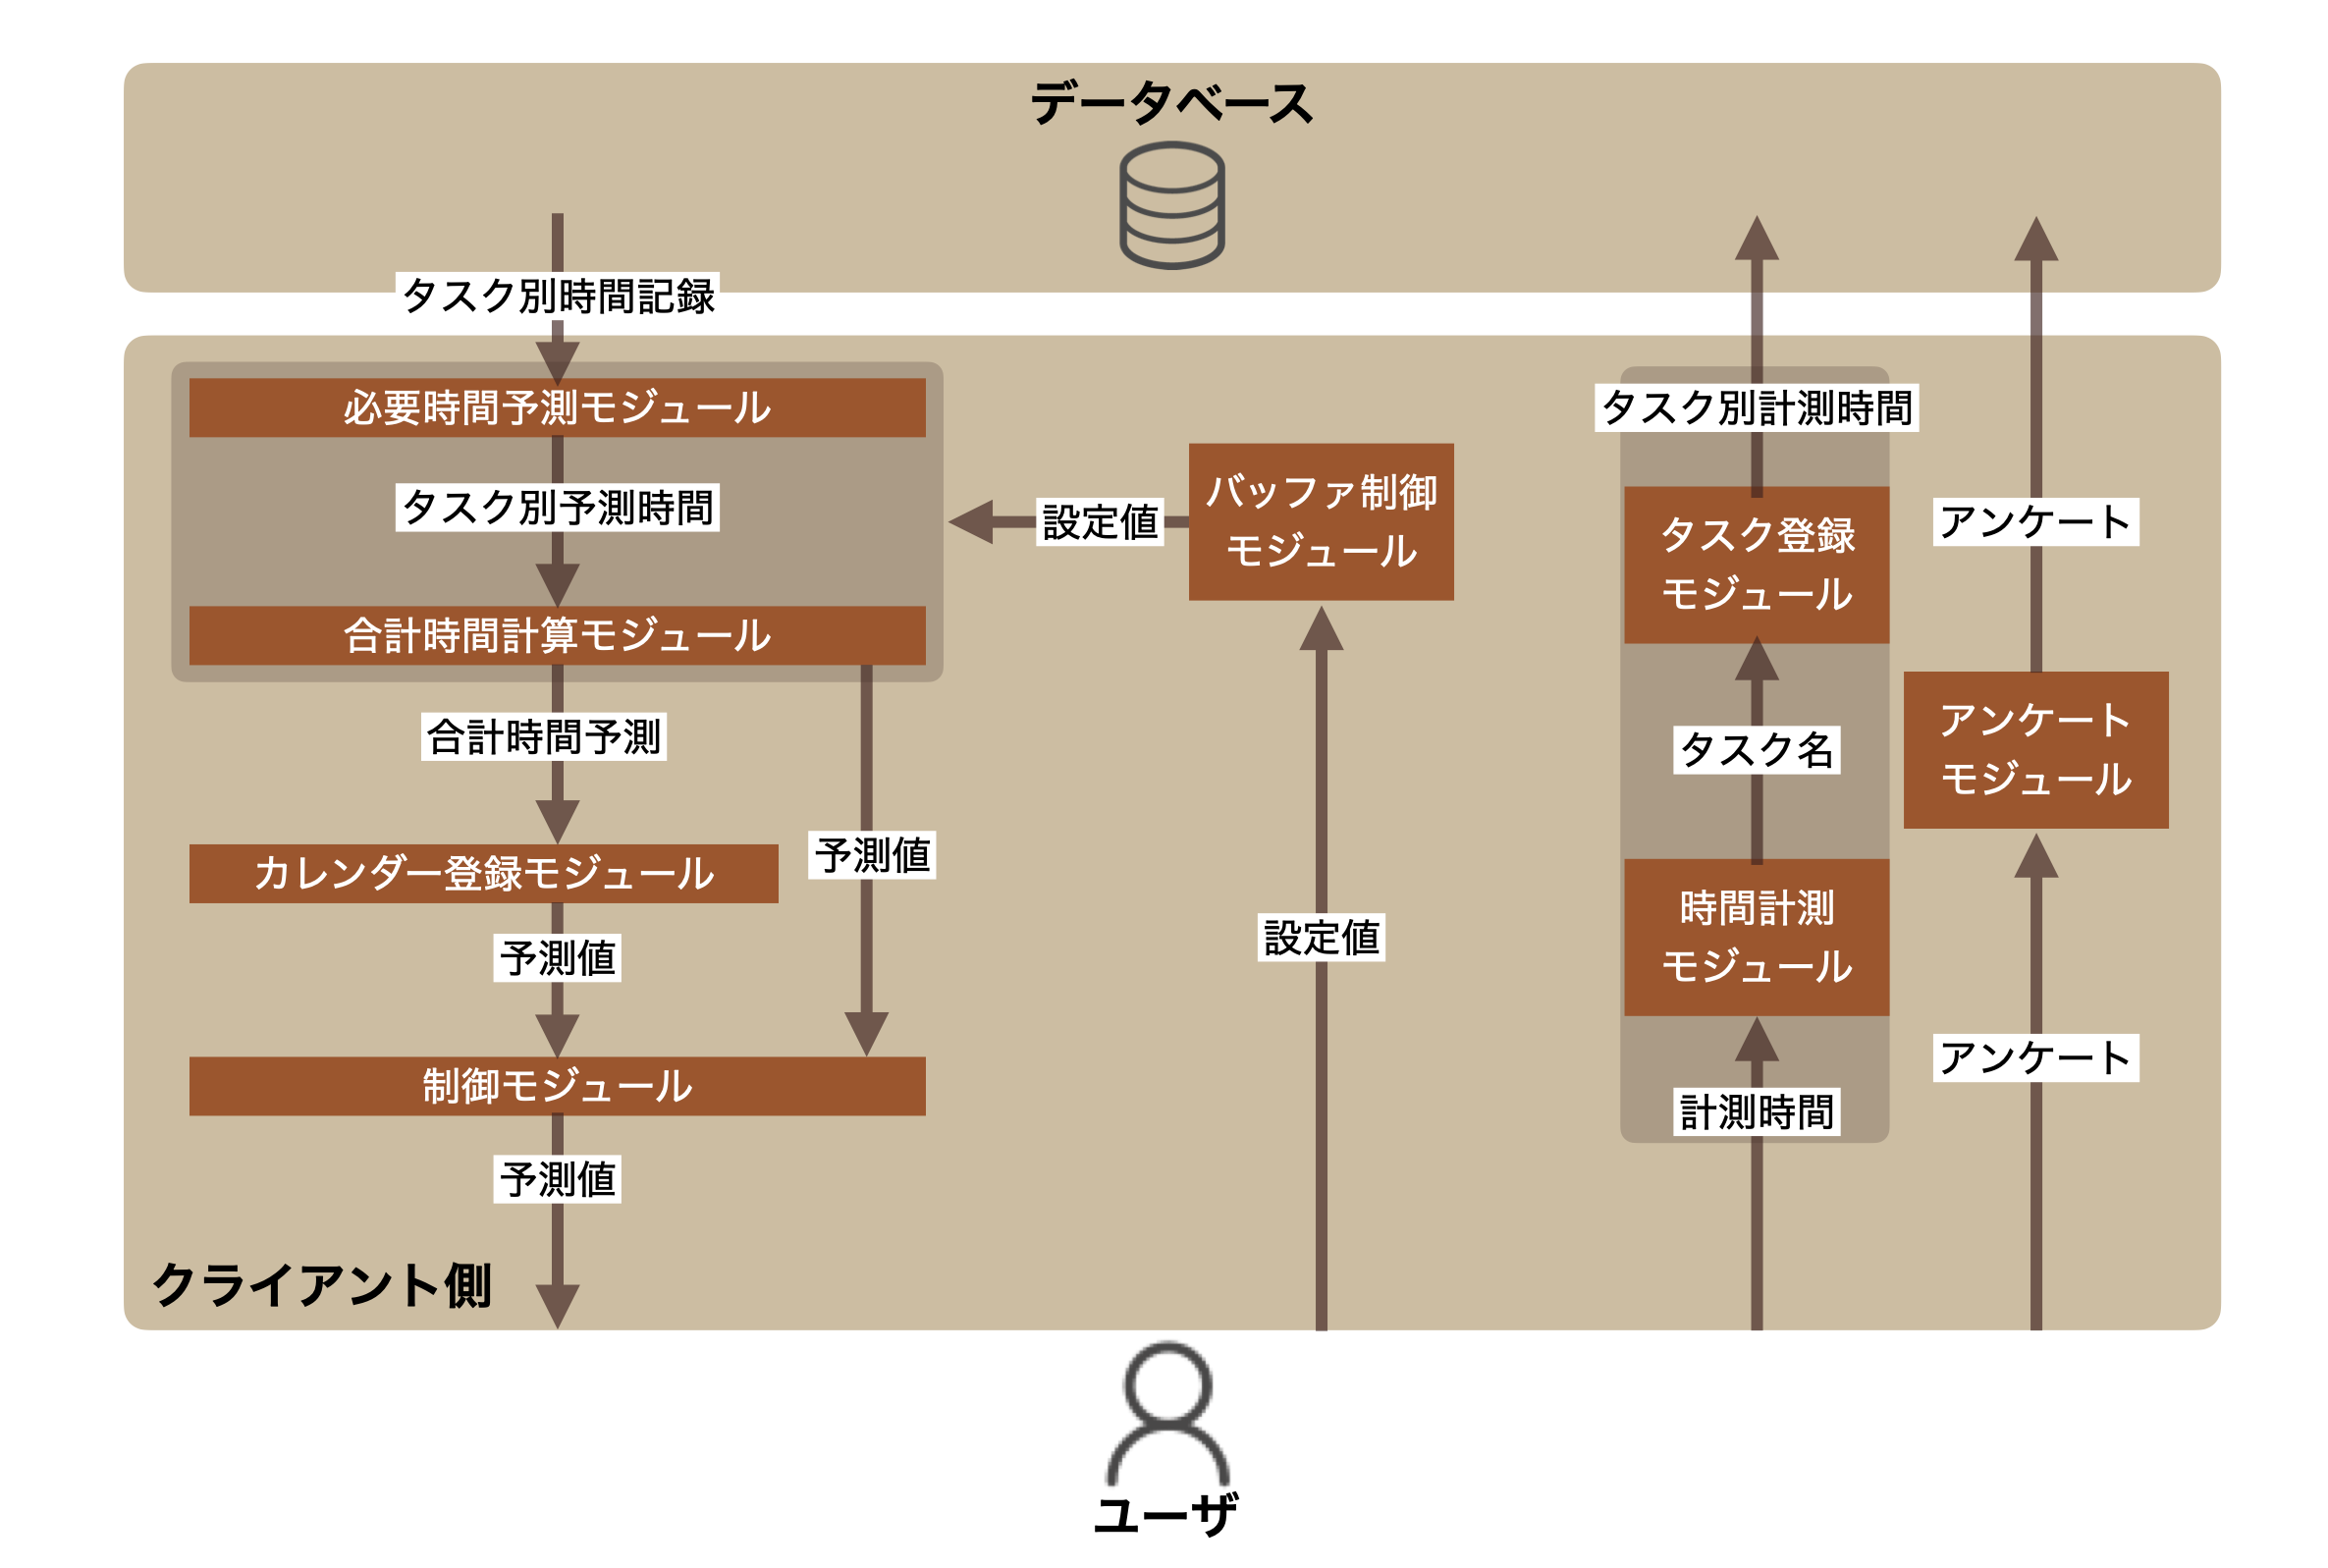
\includegraphics[width=9cm]{images/5/3.png}
	\end{center}
	\caption{システム構成図}
	\label{fig:system}
\end{figure}

\section{クライアント側設計}
本節では,クライアントであるiPhoneアプリケーションを構成する2つのモジュールについて説明する.

\subsection{タスク別時間記録モジュール}
タスク別時間記録モジュールでは,ユーザが行動した時間をタスク別に記録を行う.
ユーザは本システムをストップウォッチのとして使い時間を測定する.
行動時間測定を終了するとタスク選択画面にて行った行動を選択する.
タスク選択画面には過去入力したタスク名がリスト形式で表示されており,新規タスクである場合は新規タスク名を登録する.

\subsection{必要時間予測モジュール}
必要時間予測モジュールでは,ユーザの単一タスクないし選択された複数タスクの必要時間を予測する.
``ADLog"ボタンを押し算出画面に移動すると,タスク名毎の予測時間が自動計算されリスト形式で表示される.
リスト内のタスク名を選択すると,中央上段には選択タスクの合計必要時間が自動計算され結果が表示される.
また,同時に中央下段には合計必要時間で追加された合計バッファ時間が内訳として表示される.
それぞれの計算手法の詳細は前章にて記述した.


\section{サーバ側設計}
サーバ側ではデータベースへの書き込み及び読み込みを行う.
ユーザ別に登録タスクとタスク時間記録をサーバ内にて管理する.

\section{まとめ}
本章では,ADLoggerシステムの設計について述べた.
次章では,本システムの実装について述べる.